\documentclass[a4paper,11pt]{report}
\usepackage[utf8x]{inputenc}
\usepackage{fullpage}
\usepackage[hyphens]{url}
%\usepackage{hyperref} this messes up the line breaks of url
\usepackage{xspace}
\usepackage{listings}
\usepackage{graphicx}

% Title Page
\title{{CompLACS} Quadrotors Simulator}
\author{Renzo De Nardi,\\University College London\\\texttt{rdenardi@cs.ucl.ac.uk}}

\newcommand{\sname}{QRsim\xspace}
\newcommand{\web}{\url{http://complacs.cs.ucl.ac.uk/complacs/simulator/}\xspace}

\begin{document}
\maketitle

\begin{abstract}
This document describes the multi-vehicle quadrotor simulator (\sname) developed at UCL to devise and test algorithms for the UCL autonomous helicopters, one of the three application platforms of the {CompLACS} project.
This report is divided into two parts, the first describes the logic and the structure of the simulator while the second presents a specific example of use. 
Technical details about the dynamic models used in the simulator and their implementation are reported in the appendix. 

A companion to this report is the documentation that Matlab can automatically generate from the source code (i.e. the command \texttt{doc}), the reader is referred to it for all the more specific API details.
\end{abstract}

\tableofcontents

\chapter{Design and Concepts}

\section{Rationale}\label{sec:rationale}
UAVs provide a rich source of control problems some of which (namely the one connected with individual flight attitude control) have been successfully addressed in previous research. {CompLACS} focusses instead on the higher level problems of enabling multiple UAVs to achieve a common goal by communicating and cooperating as an autonomous flock. 

A simulator that allows to devise and test algorithms aiming at such problems must reliably model the effects that are (at least to a certain extent) common to all platforms (e.g. wind or GPS errors) as well as the interaction between them (e.g. radio communication or collisions). 
At the same time, since the real platform used in this work are already provided with off the shelf stabilisation and attitude controllers, the requirement on accurately simulating the very low level dynamic behaviour of the platform can be relaxed.
Both these sets of requirements make \sname substantially different from existing quadrotor simulator available in the literature. 


One of the objectives of {CompLACS} is to provide a generic interface to specifying learning and control problems, it is therefore important for the tools used in the initial investigation (i.e. the platforms simulators) to not be constrained to a rigid interface. 
For this reason in \sname more than providing a unique and rigid interface to the application platform, we decided to build a modular and extensible API so to make it possible to redefine the platform interface with relative ease. 

Defining concrete application scenarios based on the available platforms and simulators is one of the forthcoming deliverable of {CompLACS} (milestones 6.2, 7.2), in the following section we aim at aiding this process by giving a clear conceptual view of \sname. 

\section{Concepts}


\subsection{Platforms and Environment}\label{sec:platandenv}
Within \sname it is useful to make a logical distinction between two types of objects:
\begin{itemize}
\item platforms,
\item environment objects.
\end{itemize}
To the first type belongs the description of the quadrotor dynamics but also the models of sensors and other phenomena that are platform specific (e.g. aerodynamic turbulence). The second class comprehends al the phenomena that are not platform specific and have direct or indirect impact on several platforms (e.g. the flight area or the satellite vehicles of the GPS system).
In many ways this distinction is rather natural and in \sname we are simply exploiting it in order to provide a sensible structure to the simulator.

In general the platforms are the only objects that can be controlled by means of actions, of course those might eventually have an indirect effect on the environment. We must underline that this does not impose for any of the two classes to be time invariant, in fact both class of object might change during the course of a simulation as result of actions or simply as result of the time passing.

To the extent allowed by Matlab we used object-oriented programming in order to map physical objects directly into a corresponding class; platforms subclass the abstract class \texttt{Platform} (defined in \texttt{/src/platforms/Platform.m}) and environment objects subclass \texttt{EnvironmentObject} (defined in \texttt{/src/environment}).

\subsection{State}\label{sec:state}

At any point in time the state of the objects present in the simulator must be maintained; for reason of computational efficiency in Matlab we use a global structure to store such state. Rather obviously this data structure is called \texttt{state} and is accessible from any function or object method in the simulator.

Consistently with the definition in section \ref{sec:platandenv} we use the fields \texttt{state.environment} and the array \texttt{state.platforms} to store the handles to all the environment and platforms objects respectively. 
Given such a structure accessing the state of objects is trivial, for instance \texttt{state.platforms(1).X} gives access to the state variables of the first platform, while \texttt{state.environment.wind.direction} returns the current mean wind direction. 
The direct access to the state variables should not be used to set the state, when such an operation is meaningful (e.g. for the platforms) a specific methods (\texttt{setState(X)}) is provided by the corresponding class\footnote{In addition to overwriting the object's state these calls also make sure that 
any other internal variable (e.g. noise model states) is appropriately set.}.
The top level \texttt{Platform} and \texttt{EnvironmentObject} classes impose that derived classes must define methods to reset the state to its initial value defined by the task (see section \ref{sec:createtask}).
The reader is referred to the API documentation available through Matlab for more details on the properties of each single object.

The global state structure stores also other important variables:
\begin{itemize}
 \item the simulator time \texttt{state.t}, used to ensure synchronization between all the environment and platforms objects;
 \item the pseudorandom number generator stream \texttt{state.rStream}, used by any of the objects that requires any form of random numbers (e.g. to simulate noise samples);
 \item the simulator time step \texttt{state.DT}, the time granularity with which the simulator time is incremented;
 \item the handle to the 3D graphics visualization \texttt{state.display3d}.
\end{itemize}

\subsection{Steppable}

Since the platforms and environment that we are simulating are representation of physical objects, one natural way to think about their evolution in time is to consider time discretized into steps and to ``step forward'' the object's state at each time step. In the case of a quadrotor for instance, stepping forward is nothing more than integrating the ODE that describe its dynamics, for other object stepping forward might mean instead triggering an event associated with a specific time.
In our implementation every object that evolves with time is derived from a common class (i.e. \texttt{Steppable}) which defines an abstract \texttt{update()} method and a time step property \texttt{dt}. \texttt{update()} propagates the object's state forward to the current time \texttt{state.t}, \texttt{dt} specifies with what (time) granularity \texttt{update()} should be called. As we will see in section \ref{sec:qrobj}, the method update is never called directly, instead the  \texttt{Steppable} class exposes the method \texttt{step()} which in turns calls \texttt{update()} if a time equal to \texttt{dt} has passed since the object's state was updated\footnote{To simplify the updates the time step \texttt{dt} of any object must be a multiple of the simulator time step (\texttt{state.DT}); in practice this is not a very restrictive assumption.}.

\subsection{Task}

By combining different types of environment objects and platforms \sname allows to define a variety of single and multiple helicopter scenarios as well as many different objectives for the platforms to try to achieve. 
The abstract class \texttt{Task} provides a way to derive task objects specifying both a scenario and an activity to be learned; the class defines two main methods \texttt{init()} and \texttt{reward()}.

\texttt{init()} allows the user to define the type (i.e. the class name) of each of the environment objects as well as of each platform and sensor. 
Along with the object type, a pecification of all the class specific parameters is also needed.

The \texttt{reward()} method allows for defining an instantaneous reward for the task, this can be used for the purpose of learning. The design of a reward function is very task specific but most often the user will rely on the global \texttt{state} structure in order to compute such a reward.

\subsection{Other Abstract Classes}

At the aim of making the code easy to extend, the software API defines also several other classes to abstract the Sensors in general but more specifically the GPSreceiver, the various inertia sensors and the aerodynamic effects. This allows to configure specific type of sensor through the task object (see section \ref{sec:createtask}) instead of having to modify the platform code.

\section{The \sname Object}\label{sec:qrobj}

After a brief introduction of the fundamental building blocks of \sname we can look at they are used within the main class of the simulator. The \texttt{\sname} object allows to initialize setup and control the simulator as a whole. 

The object exposes three main methods:
\begin{itemize}
 \item \texttt{init('task\_name')}, initializes the platforms the environment objects and the task according to what specified by the task \texttt{'task\_name'} (see section \ref{sec:createtask}) and creates the \texttt{state} data structure. This is generally the first command called soon after the creation of the \texttt{\sname} object and is called only once.
 \item \texttt{reset()}, resets the simulator to the state specified in the configuration files\footnote{The parameters defined as random in the task are initialized to a new random state.}. This is generally called after a learning episode in order to restore the state of the simulator. 
 \item \texttt{step(U)}, steps in sequence all the environment object and all the platforms forward in time. This is the main command that accepts a matrix of control inputs \texttt{U} (e.g. one column array for each platform) and propagates the state of all the simulator's object. Listing \ref{lst:step} shows the implementation of the method; where it can be seen that first \texttt{state.t} is updated\footnote{This is the only statements that updates the simulation time.}, then all the environment object are propagated and only later each of the platform is stepped forward.
 After a call to step the new state can be accessed as described in section \ref{sec:state}.
 \item \texttt{reward()}, returns the instantaneous reward defined by the current task. This is meant to be called after stepping the simulator.
\end{itemize}


\begin{lstlisting}[float=ht!bp,caption=\sname step() method,language=Matlab,frame=lines,label=lst:step,numbers=left,basicstyle=\small]
function obj=step(obj,U)
  global state;
           
  %% update time
  state.t=state.t+state.DT;
                        
  %% step all the common objects
            
  % the space segment of the GPS
  state.environment.gpsspacesegment.step([]);
            
  % the wind
  state.environment.wind.step([]);
            
  %% step all the platforms            
  for i=1:length(state.platforms)
    state.platforms(i).step(U(:,i));
  end
end
\end{lstlisting}


\chapter{Installation and Use}

\section{Installation}
The simulator is entirely written in Matlab and does not depend on any additional toolbox; as a result the only requirement is a recent version of Matlab (i.e. version number greater  than 7.6)\footnote{The development and testing was carried out on R2010b for UNIX.}.
No installation as such is required, the user simply needs to download the simulator source code form \web and unpack into a directory of choice.

To use the simulator is sufficient to add its root directory (i.e. \texttt{qrsim}) to the current Matlab path; each time a \texttt{qrsim} is instantiaed any other directory needed will also be added to the curremt path.

At the aim of improving performance, some of the most computationally expensive functions in the simulator have been written also as MEX function, these can be easily compiled using the function \texttt{mexify.m}\footnote{Depending on your system setup you might need to configure the MEX compiler using \texttt{mex -setup}.}.


\section{Creating a Task}  \label{sec:createtask}

As a first example we look at a single platform task which requires to maintain the quadrotor hovering at the position it has when the task starts; the solution requires continuous control since the helicopter is affected by time varying wind disturbances. 
 
To implement such a task, we start by creating a new class that extends the abstract class \texttt{Task} and implements the \texttt{init()} and \texttt{reward()} methods.
The \texttt{init()} method (see listing \ref{lst:init}) 
\begin{lstlisting}[float=ht!bp,caption=KeepSpot init() method,language=Matlab,frame=lines,label=lst:init,numbers=left,basicstyle=\small]
function taskparams=init(obj)
 
 % Simulator step time in seconds
  taskparams.DT = 0.02;
            
  % random nmber generator seed
  taskparams.seed = 0; %if zero the seed depends on the system time         
            
  %%%%% environment %%%%%
  taskparams.environment.area.limits = [-10 20 -7 7 -20 0];
  taskparams.environment.area.type = 'BoxArea';
  [E N zone h] = lla2utm([51.71190;-0.21052;0]);
  taskparams.environment.area.originutmcoords.E = E;
  taskparams.environment.area.originutmcoords.N = N;
  taskparams.environment.area.originutmcoords.h = h;
  taskparams.environment.area.originutmcoords.zone =  zone;
  taskparams.environment.area.graphics.on = taskparams.display3d.on;
  taskparams.environment.area.graphics.type = 'AreaGraphics';
            
  % GPS
  taskparams.environment.gpsspacesegment.on = 0; 
  taskparams.environment.gpsspacesegment.dt = 0.2;
  taskparams.environment.gpsspacesegment.orbitfile = 'ngs15992_16to17.sp3';
  taskparams.environment.gpsspacesegment.tStart=%0 to initilise it randomly
  taskparams.environment.gpsspacesegment.svs=[3,5,6,7,13,16,18,19,20,22,24,29,31];
  taskparams.environment.gpsspacesegment.type = 'GPSSpaceSegmentGM';
  taskparams.environment.gpsspacesegment.PR_BETA = 2000; % process tau
  taskparams.environment.gpsspacesegment.PR_SIGMA = 0.1746; % process std
  taskparams.environment.gpsspacesegment.DT = taskparams.DT;
            
  % Wind
  taskparams.environment.wind.on = 0;
  taskparams.environment.wind.type = 'WindConstMean';
  taskparams.environment.wind.direction = 0; %0 to initilise it randomly
  taskparams.environment.wind.W6 = 0.1;  %speed 6m from ground in m/s
  taskparams.environment.wind.dt = 1;    %not in use
  taskparams.environment.wind.DT = taskparams.DT;
            
  %%%%% platforms %%%%%
  % Configuration and initial state for each of the platforms
  taskparams.platforms(1).configfile = 'pelican_config';
  taskparams.platforms(1).X = [0;0;-20;0;0;0]; 

  %%%%% visualization %%%%%
  taskparams.display3d.on = 1;
  taskparams.display3d.width = 1000;
  taskparams.display3d.height = 600;            
end
\end{lstlisting}
returns a data structure that contains general fields like the simulator time step \texttt{taskparams.DT} and the seed of the pseudorandom number generator (\texttt{taskparams.seed}), fields for each of the environment objects (\texttt{taskparams.environment}), and for each of the platforms (\texttt{taskparams.platforms}). Although the fields depend on the type of object, by convention we name:
\begin{itemize}
\item \texttt{on} the flag that allows to enable and disable the object in question,
\item \texttt{dt} the timestep of the object,
\item \texttt{type} the class nme of the object,
\item \texttt{DT} the timestep of the simulator.
\end{itemize}
The number of sensors and parameters present in a platform would make quite cumbersome defining several identical platforms; for this reason we also allow to specify as a parameter a configuration file (see \texttt{'pelican\_config'}) so that the same file can be used for more than one platform. Nonetheless is still possible to define a different initial position and orientation for each platform (see line 38).

Lastly we see the \texttt{taskparams.display3d} parameters which allow to specify if the 3D visualization is active and the size of the window used for its rendering. 

As already mentioned, a task must also define a reward function. For the task of mainitaining a fixed position in space a straightforward reward can be computed subtracting the initial position of the quadrotor from its state vector and taking the square magnitude of the vector obtained (see listing \ref{lst:reward}). 
Such a function gives higher rewards ta policy that maintain the quadrotor close to the starting point but also keeps it level (i.e. \texttt{X(4:6)=0}) and minimizes linear and rotational velocities (i.e. \texttt{X(7:12)=0});

\begin{lstlisting}[float=ht!bp,caption=KeepSpot reward() method,language=Matlab,frame=lines,label=lst:reward,numbers=left,basicstyle=\small]
function r=reward(obj)
  global state;

  e = state.platforms(1).X(1:12);
  e = e(1:3)-state.platforms(1).params.X(1:3);
  r = - e' * e; 
end
\end{lstlisting}

The complete listing for this task can be found in the file \texttt{KeepSpot.m}.  

\section{Example main}
To clarify the use of the simulator through the \texttt{\sname} object, we shall present a simple example of use; namely we will use a manually designed PID controller to achieve the behaviour required by the \texttt{KeepSpot} task.
Listing \ref{lst:main} shows the code of this bare bone example. 
\begin{lstlisting}[float=ht!bp,caption=main script,language=Matlab,frame=lines,label=lst:main,numbers=left,basicstyle=\small]
global state;

% create simulator object
qrsim = QRSim();

% load task parameters and do housekeeping
qrsim.init('KeepSpot');

% number of steps we run the simulation for
N = 3000;

for i=1:N,
    tloop=tic;    

    % compute controls
    U=quadrotorPID(state.platforms(1).eX,state.platforms(1).params.X(1:3));
    
    % step simulator 
    qrsim.step(U);

    % get reward
    % qrsim.reward();

    % wait so to run in real time
    wait = max(0,state.DT-toc(tloop));   
    pause(wait);    
end
\end{lstlisting}
Before anything else we are rquired to initialize the global structure that will hold the simulator state and give access to the quadrotor state. Next, instantiating the \texttt{\sname} object will make sure that all the functions and classes of the simulator are reacheable, is then possible to load all the task parameters by calling \texttt{qrsim.init()}. 
The main for loop drives the simulation forward by calling in sequence the PID controller and the \texttt{qrsim.step(U)} method; given the current state of the platform, the PID computes the new control action  \texttt{U} which is then used to step the dynamics forward in time.
Since we are using a PID controller and no learning is involved, after stepping the simulator we do not make use of the reward returned by the task. In the listing we show the call commented out since this is where normally it would be computed.

Since the task defines to run the simulation with the 3D visualization, it makes sense to run in real time, line 25 introduces the necessary pause.  

Finally we want to clarify that the PID controller was chosen exclusively for its simplicity, in facts it is a very consrvative controller and its performance are very much suboptimal. This said it might still be useful as a baseline for comparisons. 

\begin{center}
\begin{figure}
\label{fig:3d}
 \caption{3D visualisation}
% \includegraphics{./}
 % .: 0x0 pixel, 0dpi, 0.00x0.00 cm, bb=
\end{figure}
\end{center}

Figure \ref{fig:3d} shows a snapshot from the 3D visualisation of the simulator where both the platform and its past trajectory are visible.


\appendix
\chapter{Implementation Details}

This appendix describes in detail and provide reference to the models implemented in \sname in order to replicate a typical quadrotor platform (namely the Ascending Technologies Pelican \cite{asctec2011pelican} in use at UCL) complete of sensors.
While reading this material is not a prerequisite to use the simulator, reading it will provide in depth details about the parameters used in the various task files.

\section{Reference Frame an symbols}

For convenience we show here the body frame of reference used in many of the computation involving the helicopter dynamics (see figure \ref{fig:axes}). 
\begin{figure}[htbp]
 \begin{center}
 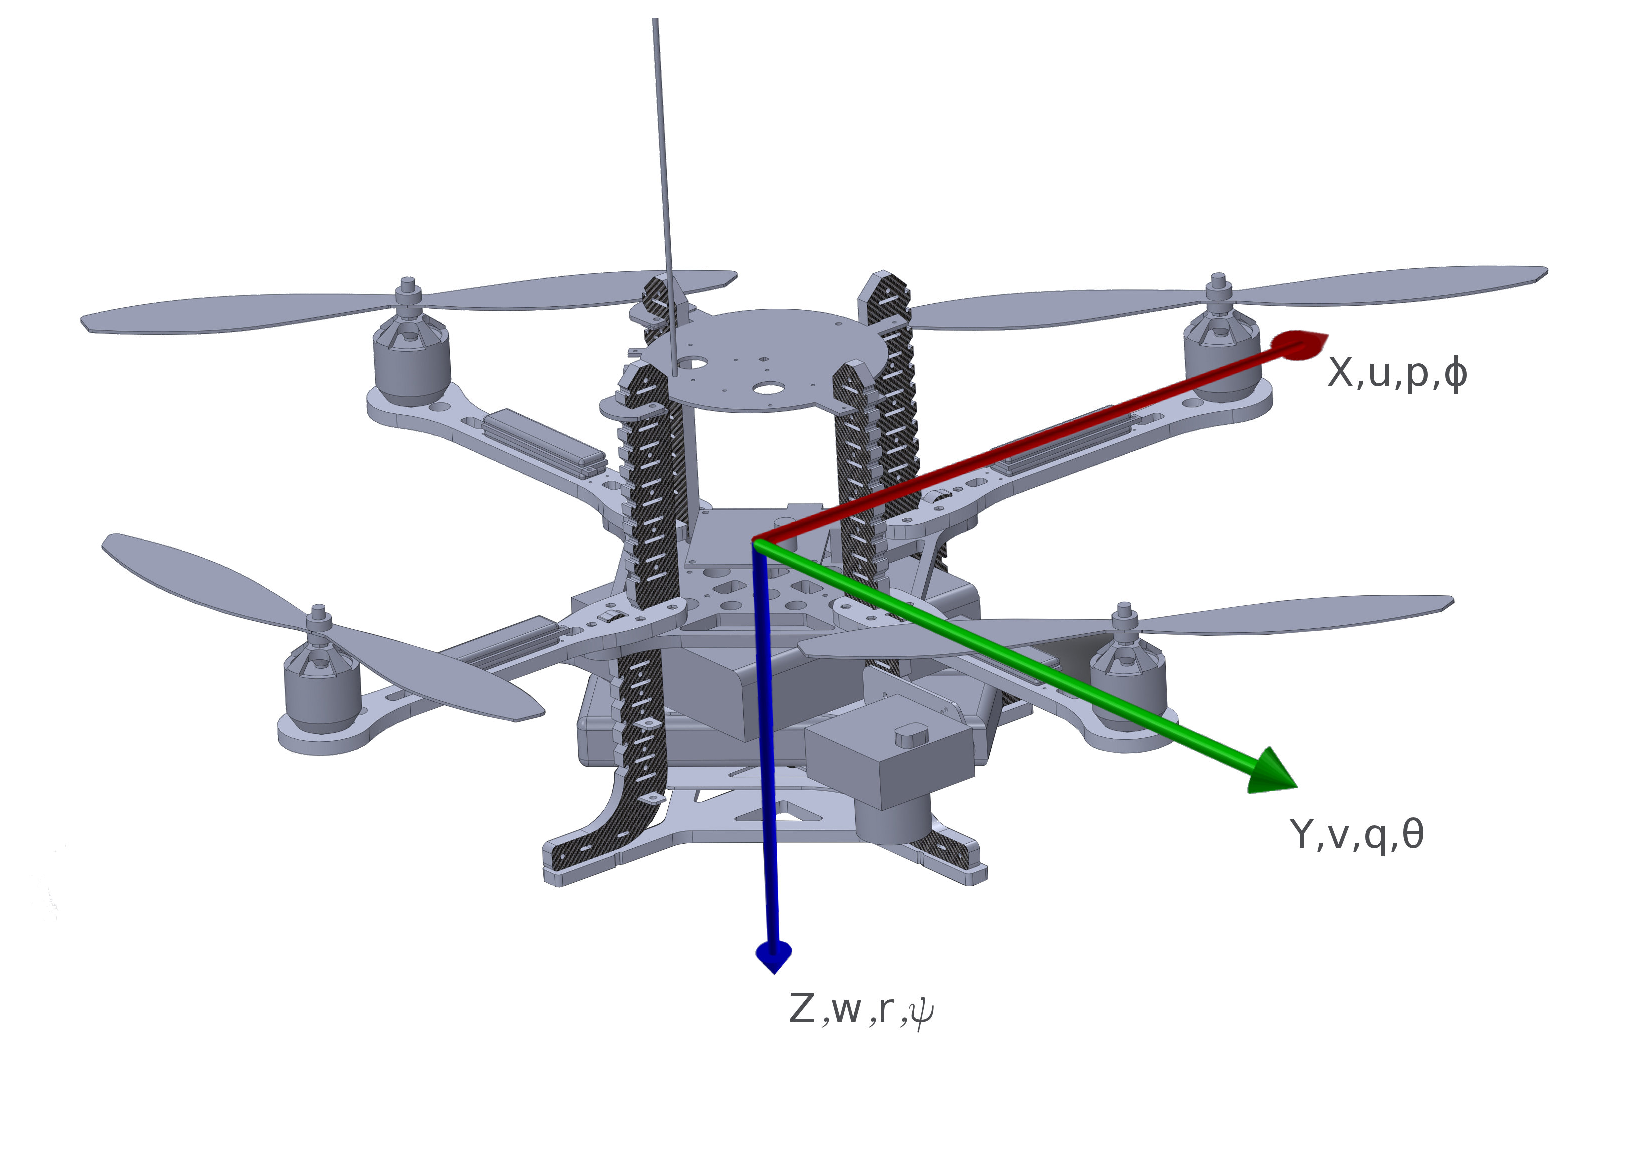
\includegraphics[width=11cm]{./axes.eps}
\caption{Body NED frame of reference and state variables.\label{fig:axes}}
\end{center}
\end{figure} 

We also define several of the variable that are used in the simulator


\section{Quadrotor dynamic model}

Several dynamic models of quadrotor helicopters based on first principles have ben published in the literature (\cite{bouabdallah07phd}, \cite{balas07modelling}, \cite{hoffmann07quadrotor}), such examples consider the forces and moments acting on the helicopter in order to obtain the rotational and translational dynamics.
These type of models replicate only the ``mechanics'' and the aerodynamics of the flying machine but do not include the action of the low level control system necessary to make the quadrotor rotational dynamics stable. Since the manufacturer of our quadrotor does not make public the design of the stabilization system, replicating it in software within the simulator is not a straightforward task. Given that the low level dynamics of the quadrotor is not our primary interest (as explained in section \ref{sec:rationale}), for the rotational dynamics we prefer to use an equivalent  model that replicates directly the combined effect of both the quadrotor dynamics and of its controller.
We learn the parameter of such a model directly from flight data in order to match as accurately as possible the characteristics of our flight machine.
For the translational dynamics we use a more standard model that consider the forces acting on the center of mass of the flight machine but we learn from data the relationship between the throttle control input and the generated thrust force since it is known to be very much dependent on the motors and propellers present on the rotorcraft.

In the case of the pitch and roll motion the Pelican platform allows to directly specify the angles that the platform should maintain, these ``desired quantities'' ($u_{pt}$ and $u_{rl}$ respectively) constitute therefore two of the control inputs. 
From flight tests we deemed that a second order model can provide a good representation of the dynamic response of the state variable $\theta$ and $\phi$ to changes in control. It was also evident that the control system controls the propeller so to limit the maximum rotational velocity (a common precaution that ensure to not exceed the sensing and/or control envelope). 

These findings are encoded in equations \ref{eqn:p} and \ref{eqn:q} where $K_{pq0}$, $K_{pq1}$ and $K_{pq2}$ are constant factors that are obtained from flight data while $p_{max}=q_{max}$ is derived from the platform firmware settings.
\begin{equation}\label{eqn:p}
\dot{p}  =  \left\{ \begin{array}{l l} K_{pq1} (K_{pq0} u_{rl} - \phi) + K_{pq2} p & |p|<p_{max} \\ 0  & |p|\geq p_{max} \end{array} \right .\\
\end{equation}
\begin{equation}\label{eqn:q}
\dot{q}  =  \left\{ \begin{array}{l l} K_{pq1} (K_{pq0} u_{pt} - \phi) + K_{pq2} q & |q|<q_{max} \\ 0  & |q|\geq q_{max} \end{array} \right .\\
\end{equation}
Perhaps quite obviously the same parameters are used for the pitch and roll dynamics since the platform is symmetric. 


The yaw motion of the platform is controlled by specifying a desired yaw speed $u_{ya}$; even in this case a second order model provides a good fit to the flight data and leads to equation \ref{eqn:r}. 
\begin{equation}\label{eqn:r}
\dot{r} = K_{r0} u_{ya} + K_{r1} r
\end{equation}
Again the constant were obtained from flight data. 

In the case of the translational dynamics the first relationship to capture is the one between the throttle control input ($u_{th}$) and the thrust force ($F_{th}$) experienced by the quadrotor. 
Through a series of static tests emerged that the relationship between throttle and thrust can be represente by a second order polynomial 
\begin{equation}
F_T = (C_{th0} + C_{th1} u_{th} + C_{th2} u^2_{th} \label{eqn:ft}
\end{equation}
 this is a typical result (\cite{denardi2010phd},\cite{hoffmann07quadrotor}) in accordance with basic lift theory which predics a lift for proportional to the blades speed.
Full throttle tests also evidenced that the maximum thrust is intimately related to the current battery voltage ($V_b$) and decreases as the battery depleats 
\begin{equation}
F_M = (C_{vb0}+C_{vb1} V_b) \label{eqn:fm}
\end{equation}.

Dynamic tests showed that due to inertia and drag effects, the thrust can not change instantanously, but instead it changes at a constant rate\footnote{We believe that this is due to the speed control loop present in the electronic speed controllers governing the motors.} $\tau_1$. Exception to this are very slow speed ranges for which a first order behaviour is exhibited instead. Combining this dynamic behaviour with the maximum thrust defined by the lowest between (\ref{eqn:ft}) and (\ref{eqn:ft}) we obtain:
\begin{equation}
\dot{F}_{th}=\left\{ \begin{array}{l l} -\tau_1 & max(F_T,F_M)<F_{th} \\ \tau_1  & max(F_T,F_M)\leqF_{th} \end{array} \right .\\
\end{equation}

Given $F_th$, the gravity force in body coordinates $g_b$ and the wind velocity in body coordinates $[u_w,v_w,w_w]$, the resulting acceleration in body coordinates can be computed as:
\begin{eqnarray}
\dot{u} &=& -q w + r v + g_b_x + K_{uv}(u-u_w)\\
\dot{v} &=& -r u + p w + g_b_y + K_{uv}(v-v_w)\\
\dot{w} & =& -p v + q u + g_b_z - \frac{F_{th}}{m} + K_w (w-w_w) l\bel{eqn:w}
\end{eqnarray}
Where $m$ is the mass of the quadrotor, and the the terms $K_{uv}(u-u_w)$,$K_{uv}(v-v_w)$ and $K_w(w-w_w)$ are the effects of the aerodynamic drag. The first two terms on the right hand side of the eqautions are result of the fact that the linear velocities $u,v,w$ are expressed in a rotation frame. 
 
Equations (\ref{eqn:p})-(\ref{eqn:w}) provide the state update equations which are numerically integrated in order to simulate the time evolution of the state variables.
The interested reader can find the implementation of the model presented in this section in the file \texttt{pelicamODE.m}.  

\section{Inertial sensors models}

On board a real quadrotor platform a series of sensors allows to produce an estimate of many of the flight variables which is very useful to control and stabilize the helicopter.
A standard suite of sensor (e.g. the one present on a \cite{asctec2011pelican}) contains a tryaxial accelerometer, a set of three gyros, a set of three magnetometers, a pressure sensor and a GPS receiver.



    % Simple barometer noise model.
    % The following assumptions are made:
    % - the noise is modelled as additive white Gaussian 
    % - the accelerometer refrence frame concides wih the body reference frame
    % - no time delays

$z_{baro}$ is output of a barometer, $h$ is true altitude, $b$ is bias noise which is modeled as first order 
Gauss-Markov process $\nu_m$ is measurement noise.
    \begin{equation}
      z_{baro}=h+b+\nu_m
      \dot{b}=-\frac{1}{\tau}b+\nu
    \end{equation}
 

Several authors have studied the 

Since in our platform the low level stabilization is performed on board and is not of interest for the type of activity considered in CompLACS, at this instance we are not planning to make direct use of the accelerometers and gyros reading. We decided therefore

The modular nature of the simulator will allow to easily upgrade to a more complex noise model if this is deemed necessary.   

    % Simple accelerometer noise model.
    % The following assumptions are made:
    % - the noise is modelled as an additive Gauss-Markov process. 
    % - the accelerometer refrence frame concides wih the body reference frame
    % - no time delays

    % Simple gyroscope noise model.
    % The following assumptions are made:
    % - the noise is modelled as additive white Gaussian. 
    % - the accelerometer refrence frame concides wih the body reference frame
    % - no time delays

    % Simple orientation noise model.
    % The following assumptions are made:
    % - the noise is modelled as an additive Gauss-Markov process. 
    % - the accelerometer refrence frame concides wih the body reference frame
    % - no time delays

The orientation of the flying mchine is generally estimated on-board using primarily the input from gyros and accelerometers and magnetometers, but in some cases might also include  other sensors (i.e. the GPS and barometer). Since all these sensors are combined using an estimator (e.g. a Kalman filter), designing a noise model for the orientation measurement is all but trivial. In our case matters are further complicated by the fact that the manufacturer does not make available in depth information about the attitude estimator.
 
Pragmatically we decide to go for a much simpler noise model that attempts to capture the main characteristic of the errors in the estimated attitude. 
high acceleration where the simplification often adopten in the mechanizaion equation of the estimator introduce some level of error. 

Ornstein–Uhlenbeck process

\section{GPS model}
            % constructs the object.
            % Selects the satellite vehicles visible to this receiver among the ones in
            % objparams.svs the total number of visible satellites is generate
            % randomly (uniform number between objparams.minmaxnumsv(1) and
            % objparams.minmaxnumsv(2)). The selection of satellites is kept FIX during
            % all the simulation.
    % Class that simulates the correlate noise affecting the GPS pseudorange.
    % The running assumption is that all the receivers are (approximately) geographically
    % co-located so that pseudorange measurements to the same satellite vehicle obtained
    % by different receivers are strongly correlated.
    %
    % At each epoch the position of each satellite vehicles is determined interpolating
    % the precise orbits file (SP3) defined in params.environment.gpsspacesegment.preciseorbitfile,
    % pseudorange errors are considered additive and modelled by a Gauss-Markov process [1][2].
    % Global variables are used to maintain the noise states shared between receivers.
    %
    % [1] J. Rankin, "An error model for sensor simulation GPS and differential GPS," IEEE
    %     Position Location and Navigation Symposium, 1994, pp.260-266.
    % [2] Carlson, Justin, "Mapping Large, Urban Environments with GPS-Aided SLAM" (2010).
    %     Dissertations. Paper 44.

\section{Wind model}
    % Linear Turbulence model according to U.S. military specification MIL-F-8785C
    %
    % According to references[1, 2], turbulence can be modelled as a stochastic process
    % defined by velocity spectra. The turbulence field is assumed to be "frozen" in time
    % and space (i.e.: time variations are statistically equivalent to distance variations
    % in traversing the turbulence field). This assumption implies that the turbulence-induced 
    % responses of the aircraft is result only of the motion of the aircraft relative to 
    % the turbulent field (i.e. w = Omega * V).
    % 
    % MILF8785-C specifies both linear and rotational components of the
    % turbulence however this class currently implements only the linear disturbences.
    % The turbulence axes orientation in this region is defined as being aligned with
    % the reletive wind direction.
    %
    %
    % AerodynamicTurbulenceMILF8785 Properties:
    %    Z0                         - reference height (Constant)
    %
    % AerodynamicTurbulenceMILF8785 Methods:
    %    AerodynamicTurbulenceMILF8785(objparams)   - constructs the object an sets its
    %                                                 main fields
    %    getLinear(state)           - returns the linear component of the turbulence
    %    getRotational(state)       - always returns zero since this model does not have
    %                                 a rotational wind component
    %    update(XandWind)           - updates the GM turbulence model
    %
    %
    % [1] "Military Specification, “Flying Qualities of Piloted Airplanes" Tech. Rep.
    %      U.S. Military Specification MIL-F-8785C.
    % [2] "Creating a Unified Graphical Wind Turbulence Model from Multiple Specifications"
    %      Stacey Gage
    % [3] "Wind Disturbance Estimation and Rejection for Quadrotor Position Control"
    %     Steven L. Waslander, Carlos Wang

\bibliography{manual}
\bibliographystyle{plain}
\end{document}          
